\حصہ{سوالات مشین، امالی مشین}
%=============
\ابتدا{سوال}
چار قطب امالی موٹر \عددیء{50} ہرٹز کی \عددیء{415} وولٹ برقی دباو پر پورا بوجھ اٹھاتے ہوئے \عددیء{1455} چکر فی منٹ کی رفتار سے گھوم رہی ہے۔
\begin{itemize}
\item
موٹر کی سرک \عددیء{s} حاصل کریں۔
\item
گھموتے لچھے میں برقی رو کی تعدد حاصل کریں۔
\item
ساکن لچھے کے مقناطیسی دباو کے موج کی رفتار ساکن لچھے کی نسبت سے حاصل کریں۔
\item
ساکن لچھے کے مقناطیسی دباو کے موج کی رفتار گھومتے لچھے کی نسبت سے حاصل کریں۔
\item
گھومتے لچھے کے مقناطیسی دباو کے موج کی رفتار ساکن لچھے کی نسبت سے حاصل کریں۔
\item
گھومتے لچھے کے مقناطیسی دباو کے موج کی رفتار گھومتے لچھے کی نسبت سے حاصل کریں۔
\end{itemize} 

جوابات:\عددیء{0.03}، \عددیء{\SI{1.5}{\hertz}}، \عددیء{1500} چکر فی منٹ، \عددیء{45} چکر فی منٹ، \عددیء{1500} چکر فی منٹ، \عددیء{45} چکر فی منٹ۔
\انتہا{سوال}
%===============

\ابتدا{سوال}
موٹر کے دھرے پر چند چکر کا پیمائشی لچھا نسب کرتے ہوئے گھومتے لچھے میں پیدا برقی دباو  کی تعدد دریافت کی جا سکتی ہے۔مقناطیسی قالب سے باہر پائے جانے والا غیر مطلوب مقناطیسی بہاو اس لچھے میں برقی دباو پیدا کرتا ہے۔ایسے ہی ایک پیمائشی لچھے میں \عددیء{\SI{0.55}{\hertz}} تعدد  کی برقی دباو پیدا ہوتی ہے۔اگر یہ چار قطب والا موٹر \عددیء{\SI{50}{\hertz}} کی بجلی سے چل رہا ہو تب موٹر کی سرک اور رفتار حاصل کریں۔

 جوابات:موٹر کی سرک \عددیء{\tfrac{0.55}{50}=0.011} ہے۔معاصر رفتار \عددیء{\tfrac{2}{4} \times 50 \times 60=1500} چکر فی منٹ ہے۔یوں موٹر کی رفتار \عددیء{1500(1-0.011)=1483.5}  چکر فی منٹ ہے۔
\انتہا{سوال}
%========
\ابتدا{سوال}\شناخت{سوال_امالی_ریل_گاڑی_الف}
ایک بے بوجھ امالی موٹر \عددیء{50} ہرٹز کی بجلی پر \عددیء{1498} چکر فی منٹ کے رفتار سے گھومتی ہے جبکہ پورے بوجھ پر اس کی رفتار  \عددیء{1395} چکر فی منٹ ہوتی ہے۔
\begin{itemize}
\item
موٹر کی معاصر رفتار حاصل کریں۔ 
 \item
یہ موٹر کتنے قطب کی ہے؟
\item
بے بوجھ اور پورے بوجھ پر موٹر کی سرک حاصل کریں۔
\item
اگر گومتے حصے کا رداس \عددیء{\SI{15}{\centi \meter}} ہو تب پورے بوجھ پر رادس پر پائے جانے والا نقطہ کس رفتار سے حرکت کرت ہے۔ 
\end{itemize}

جوابات:
\begin{itemize}
\item
پچاس ہرٹز کے بجلی سے دو قطب والے موٹر کی معاصر رفتار \عددیء{3000} چکر فی منٹ جبکہ چار قطب موٹر کی \عددیء{1500} چکر فی منٹ اور چہ قطب والے موٹر کی \عددیء{1000} چکر فی منٹ ہو گی۔بے بوجھ موٹر تقریباً معاصر رفتار سے چلتی ہے لہٰذا موجودہ سوال میں موٹر کی معاصر رفتار \عددیء{1500} چکر فی منٹ ہے۔
\item
موٹر کے چار قطب ہیں۔
\item
بے بوجھ سرک \عددیء{\tfrac{1500-1498}{1500}=0.00133} جبکہ پورے بوجھ پر سرک \عددیء{\tfrac{1500-1395}{1500}=0.07} ہے۔ ان جوابات کو \عددیء{0.133\%} اور \عددیء{7\%} بھی لکھا جا سکتا ہے۔
\item
گھومتے حصے کی گولائی \عددیء{2 \times \pi \times 0.15=\SI{0.94248}{\meter}} ہے۔موٹر  \عددیء{1395 \times 60=\num{83700}} چکر فی گھنٹا گھومتی ہے۔یوں رداس پر پائے جانے والا نقطہ \عددیء{\tfrac{83700 \times 0.94248}{1000}=\SI{79}{\kilo \meter \per \hour}} کی رفتار سے حرکت کرے گا۔
\end{itemize}
\انتہا{سوال}
%============
\ابتدا{سوال}
امالی موٹر کے  ساکن لچھے کو سیدھا کرتے ہوئے  برقی ریل گاڑی پر نسب کر کے اور ریل کے پٹڑی کو پنجرا نما بناتے ہوئے برقی ریل گاڑی بنائی جاتی ہے۔گاڑی پر نسب لچھوں کو ریل کے پٹڑی کے ساتھ ساتھ چلتی برقی تاروں سے سرک چھلوں کے ذریعہ برقی طاقت مہیا کی جاتی ہے۔تین مرحلہ، سولہ قطب کے لچھوں کو گاڑی میں سیدھی سطح پر کُل چار میٹر لمبائی پر نسب کیا جاتا ہے جبکہ اس کو پچاس ہرٹز کی بجلی فراہم کی جاتی ہے۔
\begin{itemize}
\item
گاڑی کی معاصر رفتار حاصل کریں۔
\item
اگر گاڑی \عددیء{\SI{85}{\kilo \meter \per \hour}} کی رفتار سے جل رہی ہو تب سرک حاصل کریں۔
\item
سرک تبدیل کئے بغیر گاڑی کو \عددیء{\SI{150}{\kilo \meter \per \hour}} کی رفتار پر چلانے کی خاطر درکار تعدد حاصل کریں۔ 
\end{itemize}   

جوابات:
\begin{itemize}
\item
سوال \حوالہ{سوال_امالی_ریل_گاڑی_الف} کو دوبارہ دیکھیں۔یہاں موٹر کا ایک چکر چار میٹر کے برابر ہے جبکہ معاصر رفتار \عددیء{\tfrac{2}{16} \times 50=6.25} چکر فی سیکنڈ ہے۔یوں سیدھی معاصر رفتار \عددیء{6.25 \times 4=\SI{25}{\meter \per \second}} یا \عددیء{\SI{90}{\kilo \meter \per \hour}} ہے۔ 
\item
سرک \عددیء{\tfrac{90-85}{90}=0.0555} یعنی \عددیء{5.555 \%} ہے۔
\item
سرک \عددیء{0.0555} اور گاڑی کی رفتار \عددیء{\SI{150}{\kilo \meter \per \hour}}  کا مطلب ہے کہ معاصر رفتار \عددیء{\tfrac{150}{1-0.0555}=\SI{158.81}{\kilo \meter \per \hour}} یعنی \عددیء{\SI{44.115}{\meter \per \second}} ہے  جو  \عددیء{\tfrac{44.115}{4}=11.029} چکر فی سیکنڈ معاصر رفتار کے مترادف ہے۔یوں درکار تعدد \عددیء{\tfrac{16}{2} \times 11.029=\SI{88.23}{\hertz}} ہے۔
\end{itemize}
\انتہا{سوال}
%==============
\ابتدا{سوال}
تین مرحلہ، دو قطب والی ستارہ  امالی موٹر \عددیء{\SI{50}{\hertz}} اور \عددیء{\SI{415}{\volt}} پر چلائی جاتی ہے۔موٹر کے مساوی اجزاء مندرجہ ذیل ہیں۔
\begin{align*}
R_s=0.182, \quad X_s=0.453,\quad R_r'=0.138,\quad X_r'=0.213,\quad R_c=215.07,\quad X_m=15.51
\end{align*}
موٹر کی رفتار، داخلی اور خارجی طاقت،کارکردگی، قوت گردشہ، اور جزو طاقت ایک فی صد، دو فی صد اور تین فی صد سرک پر حاصل کریں۔

جوابات:\عددیء{s=0.01} پر \عددیء{990} چکر فی منٹ، \عددیء{\SI{12.477}{\kilo \watt}}، \عددیء{\SI{11.333}{\kilo \watt}}، \عددیء{90.8 \%}، \عددیء{\SI{109.31}{\newton \meter}} اور \عددیء{0.747} ہوں گے۔\عددیء{s=0.02} پر \عددیء{980} چکر فی منٹ، \عددیء{\SI{23.667}{\kilo \watt}}، \عددیء{\SI{21.755}{\kilo \watt}}، \عددیء{91.9 \%}، \عددیء{\SI{211.98}{\newton \meter}} اور \عددیء{0.885} ہوں گے۔\عددیء{s=0.03} پر \عددیء{970} چکر فی منٹ، \عددیء{\SI{34.339}{\kilo \watt}}، \عددیء{\SI{31.209}{\kilo \watt}}، \عددیء{90.9 \%}، \عددیء{\SI{307.23}{\newton \meter}} اور \عددیء{0.919} ہوں گے۔

\انتہا{سوال}
%=============

\ابتدا{سوال}
تین مرحلہ امالی موٹر  جسے درکار تعدد کی برقی دباو فراہم کی جائے، چالو ہوتے وقت \عددیء{155} فی صد اور زیادہ سے زیادہ \عددیء{240} فی صد قوت گردشہ پیدا کرتا ہے جہاں اس کی سکت \عددیء{100} فی صد ہے۔ ساکن لچھے کی مزاحمت اور قالبی ضیاع مزاحمت \عددیء{R_c} کو نظرانداز کرتے ہوئے مندرجہ ذیل حاصل کریں۔
\begin{itemize}
\item
زیادہ سے زیادہ قوت گردشہ پر سرک۔
\item
سو فی صد قوت گردشہ پر سرک۔
\item
سو فی صد بوجھ پر گھومتے لچھے کی برقی رو کی نسبت سے چالو کرتے وقت گھومتے لچھے کی برقی رو۔
\end{itemize}

حل:
\begin{itemize}
\item
مزاحمت \عددیء{R_s} اور \عددیء{R_c} نظرانداز کرتے ہوئے  مساوات \حوالہ{مساوات_امالی_تھونن_متغرات} سے  \عددیء{Z_t=\tfrac{X_s X_m}{X_s+X_m} =X_t} یعنی \عددیء{R_t=0} حاصل ہوتا ہے۔یوں زیادہ سے زیادہ پروڑ مساوات \حوالہ{مساوات_امالی_زیادہ_طاقت_پر_سرک} کے مطابق  \عددیء{s_z=\tfrac{R_r'}{X_t+X_r'}} سرک پر حاصل ہو گا۔چالو ہوتے وقت سرک کی قیمت ایک ہوتی ہے لہٰذا مساوات \حوالہ{مساوات_امالی_تین_دور_مروڑ_الف} میں \عددیء{s=1} پُر کرتے ہوئے چالو ہوتے وقت کی قوت گردشہ \عددیء{T_{s=1}} حاصل کی جا سکتی ہے جبکہ مساوات \حوالہ{مساوات_امالی_زیادہ_سے_زیادہ_مروڑ} میں \عددیء{R_t=0} پُر کرتے ہوئے \عددیء{T_z=\tfrac{1}{\omega_{sm}} \tfrac{3 V_t^2}{2(X_t+X_r')}} لکھا جائے گا۔یوں
\begin{align*}
\frac{T_z}{T_{s=1}}=\frac{240}{155}=\frac{R_r'^2+\left(X_t+X_r' \right)^2}{2 R_r' (X_t+X_r')}=\frac{s_z^2+1}{2 s_z}
\end{align*}
حاصل ہوتا ہے جہاں آخری قدم پر \عددیء{R_r'=s_z (X_t+X_r')} پُر  کیا گیا۔اسے حل کرتے ہوئے  جوابات \عددیء{s_z=2.73}  اور \عددیء{s_z=0.36625} میں سے زیادہ سے زیادہ قوت گردشہ پر   \عددیء{s_z=0.36625}  درست جواب چنا جاتا ہے چونکہ \عددیء{s_z=2.73} پر مشین بطور بریک کام کرے گی۔
\item
بالکل مندرجہ بالا کی طرح پوری طاقت پر سرک \عددیء{s} لکھتے ہوئے ہم لکھ سکتے ہیں۔
\begin{align*}
\frac{T_z}{T}=\frac{240}{100}=\frac{\frac{R_r'^2}{s^2}+\left(X_t+X_r' \right)^2}{2 \frac{R_r'}{s} (X_t+X_r')}=\frac{\frac{s_z^2}{s^2}+1}{2 \frac{s_z}{s}}
\end{align*}
جوابات \عددیء{\tfrac{s_z}{s}=4.5817} اور \عددیء{\tfrac{s_z}{s}=0.21825} سے  درست جواب \عددیء{\tfrac{s_z}{s}=4.5817} چنا جاتا ہے چونکہ زیادہ سے زیادہ قوت گردشہ سو فی صد قوت گردشہ کے سرک سے زیادہ سرک پر حاصل ہوتی ہے۔یوں کُل قوت گردشہ پر سرک \عددیء{\tfrac{0.36625}{4.5817}=0.0799} ہو گی۔
\item
مساوات \حوالہ{مساوات_امالی_گھمتا_رو} سے چالو کرتے وقت \عددیء{s=1}  لکھتے ہوئے
\begin{align*}
\frac{I_{r\textup{چالو}}'}{I_{r\textup{کل}}'}=\frac{\sqrt{\frac{R_r'^2}{s^2}+(X_t+X_r')^2}}{\sqrt{R_r'^2+(X_t+X_r')^2}}=\frac{\sqrt{\frac{s_z^2}{s^2}+1}}{\sqrt{s_z^2+1}}=\frac{\sqrt{4.5817^2+1}}{\sqrt{0.36625^2+1}}=4.4
\end{align*}
حاصل ہوتا ہے۔یوں چالو کرتے وقت پوری طاقت کے وقت درکار برقی رو کے \عددیء{440} فی صد برقی رو ہو گی۔

\end{itemize}
\انتہا{سوال}
%====================

\ابتدا{سوال}
ایک پنجرا نما امالی موٹر \عددیء{7.2} فی صد سرک پر پورا بوجھ اٹھاتا ہے جبکہ \عددیء{43} فی صد سرک پر \عددیء{215} فی صد کا زیادہ سے زیادہ قوت گردشہ پیدا کرتا ہے۔چالو کرتے وقت کی قوت گردشہ کُل بوجھ کی نسبت سے حاصل کریں۔

حل:مساوات \حوالہ{مساوات_امالی_تین_دور_مروڑ_الف} اور  مساوات \حوالہ{مساوات_امالی_زیادہ_سے_زیادہ_مروڑ} سے
\begin{align*}
\frac{T_z}{T}=\frac{215}{100}=\frac{2 R_t \frac{R_r'}{s}+\frac{R_r'^2}{s^2}+R_t^2+(X_t+X_r')^2}{2 \left(\frac{R_r'}{s}\right)(R_t+\sqrt{R_t^2+(X_t+X_r')^2})}
\end{align*}
حاصل ہوتا ہے۔مساوات \حوالہ{مساوات_امالی_زیادہ_طاقت_پر_سرک} کی مدد سے اسے یوں لکھا جا سکتا ہے۔
\begin{align*}
2.15=\frac{2 R_t \left(\frac{R_r'}{s}\right)+\frac{R_r'^2}{s^2}+\frac{R_r'^2}{s_z^2}}{2 \left(\frac{R_r'}{s}\right)(R_t+\frac{R_r'}{s_z})}=\frac{\frac{2}{s} \left(\frac{R_t}{R_r'}\right) +\frac{1}{s^2}+\frac{1}{s_z^2}}{\frac{2}{s} (\frac{R_t}{R_r'}+\frac{1}{s_z})}
\end{align*}
اس میں \عددیء{s_z=0.43} اور \عددیء{s=0.072} پُر کرتے ہوئے \عددیء{\tfrac{R_t}{R_r'}=1.8597} حاصل ہوتا ہے۔چالو کرتے وقت \عددیء{s=1} لیتے ہوئے مساوات \حوالہ{مساوات_امالی_تین_دور_مروڑ_الف} کی مدد سے 
\begin{align*}
\frac{T_\textup{چالو}}{T}&=\frac{s\left[(R_t+\frac{R_r'}{s})^2+(X_t+X_r')^2 \right]}{(R_t+R_r')^2+(X_t+X_r')^2}\\
&= \frac{s\left[(\frac{R_t}{R_r'}+\frac{1}{s})^2+\left(\frac{X_t+X_r'}{R_r'}\right)^2 \right]}{(\frac{R_t}{R_r'}+1)^2+\left(\frac{X_t+X_r'}{R_r'}\right)^2}
\end{align*}
لکھا جا سکتا ہے جسے مساوات \حوالہ{مساوات_امالی_زیادہ_طاقت_پر_سرک} کی مدد سے یوں لکھ سکتے ہیں۔
\begin{align*}
\frac{T_\textup{چالو}}{T}&= \frac{s\left[(\frac{R_t}{R_r'}+\frac{1}{s})^2+\frac{1}{s_z^2}-\left(\frac{R_t}{R_r'}\right)^2 \right]}{(\frac{R_t}{R_r'}+1)^2+\frac{1}{s_z^2}-\left(\frac{R_t}{R_r'}\right)^2 }
\end{align*}
لکھا جا سکتا ہے جس میں پوری طاقت کی سرک \عددیء{s=0.072}، زیادہ سے زیادہ قوت گردشہ پر سرک \عددیء{s_z=0.43} اور \عددیء{\tfrac{R_t}{R_r'}} کی قیمت پُر کرتے ہوئے
\begin{align*}
\frac{T_\textup{چالو}}{T}&= \frac{0.072\left[(1.8597+\frac{1}{0.072})^2+\frac{1}{0.43^2}-\left(1.8597\right)^2 \right]}{(1.8597+1)^2+\frac{1}{0.43^2}-\left(1.8597\right)^2 }=1.7771
\end{align*}
حاصل ہوتا ہے۔ یوں \عددیء{T_{\textup{چالو}}=1.7771 T_{\textup{پورا بوجھ}}} ہو گا۔
\انتہا{سوال}
%===============================
\begin{figure}
\centering
%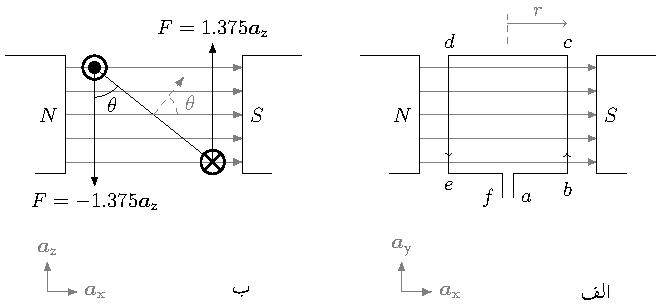
\includegraphics{figEnergyConversionTorqueOnOneTurn}
\begin{tikzpicture}
%grid
%\draw[gray,thick] (-0.5,-0.5) grid (2,2);
%\draw[gray,thin,xstep=0.1,ystep=0.1] (-0.5,-0.5) grid (2,2);
\pgfmathsetmacro{\rad}{1}
 \pgfmathsetmacro{\len}{2}
\pgfmathsetmacro{\gap}{0.5}
%defining mid point arrow macros
\tikzset{->-/.style={decoration={
  markings,
  mark=at position #1 with {\arrow{>}}},postaction={decorate}}}
\tikzset{-<-/.style={decoration={
  markings,
  mark=at position #1 with {\arrow{<}}},postaction={decorate}}}
%
%flux
\foreach \y in {0.1,0.3,0.5,0.7,0.9}{
\draw[gray,thin,-latex](-\rad-\gap,\y*\len)--(\rad+\gap,\y*\len);
}
%coil as Dot and Cross
\draw[thick](\rad,0.7*\len) circle (0.2);
\draw[thick](\rad,0.7*\len)++(-135:0.2)--++(45:0.4);
\draw[thick](\rad,0.7*\len)++(135:0.2)--++(-45:0.4);
\draw[thick](-\rad,0.3*\len) circle (0.2);
\draw[fill](-\rad,0.3*\len) circle (0.1);
%torque and moment arm
\draw[-latex](\rad,0.7*\len)coordinate (kCross)--++(0,-\len)node[below]{$F_{bc}=-1.375 \az $};
\draw[-latex](-\rad,0.3*\len) coordinate(kDot)--++(0,\len)node [above]{$F_{de}=1.375 \az $};
\draw(\rad,0.7*\len)--(-\rad,0.3*\len)coordinate [pos=0.5](kO);
%perpendicular
%\draw[gray,dashed,-latex] (kO)--($(kO)!0.8cm!90:(\rad,0.9*\len)$)coordinate [pos=0.5](kA);
%angle
\draw([shift={(90:0.5)}]-\rad,0.3*\len) arc (90:20:0.5);
\draw(-\rad,0.3*\len)++(55:0.7)node[]{$\theta$};
%magnet
\draw(-\rad-2*\gap,0)--++(1*\gap,0)--++(0,\len)node[left,pos=0.5]{$N$}--++(-\rad,0);
\draw(\rad+2*\gap,0)--++(-1*\gap,0)--++(0,\len)node[right,pos=0.5]{$S$}--++(\rad,0);
%unit vectors
\draw[-latex,gray](-1.8,-2)--++(0.5,0)node[right]{$\ax$};
\draw[-latex,gray](-1.8,-2)--++(0,0.5)node[above]{$\az$};
\draw node at (1.5,-2){ب};
%
%
\begin{scope}[xshift=6cm]
%flux
\foreach \y in {0.1,0.3,0.5,0.7,0.9}{
\draw[gray,thin,-latex](-\rad-\gap,\y*\len)--(\rad+\gap,\y*\len);
}
%coil top view
\draw [->-=0.192,->-=0.815] (0.1,-0.4)node[right]{$a$}--++(0,0.4)--++(\rad-0.1,0)node[below]{$b$}--++(0,\len)node[above]{$c$}--++(-2*\rad,0)node[above]{$d$}--++(0,-\len)node[below]{$e$}--++(\rad-0.1,0)--++(0,-0.4)node[left]{$f$};
\draw[gray,dashed] (0,1.1*\len)--++(0,0.5); 
\draw[gray,->] (0,1.1*\len+0.35)--++(\rad,0)node[above,pos=0.5]{$r$};
%magnet
\draw(-\rad-2*\gap,0)--++(1*\gap,0)--++(0,\len)node[left,pos=0.5]{$N$}--++(-\rad,0);
\draw(\rad+2*\gap,0)--++(-1*\gap,0)--++(0,\len)node[right,pos=0.5]{$S$}--++(\rad,0);
%unit vectors
\draw[-latex,gray](-1.8,-2)--++(0.5,0)node[right]{$\ax$};
\draw[-latex,gray](-1.8,-2)--++(0,0.5)node[above]{$\ay$};
\draw node at (1.5,-2){الف};
%
\end{scope}
\end{tikzpicture}%
%\caption{ایک چکر کے لچھے پر قوت اور قوت مروڑ}
%\label{شکل_تبادلہ_طاقت_لچھے_پر_قوت_اور_مروڑ}
\end{figure}
